\documentclass[11pt,a4paper,titlepage,parskip=half]{scrreprt}

\usepackage[utf8x]{inputenc}
\usepackage[ngerman]{babel}
\usepackage{ucs}
\usepackage{amsmath}
\usepackage{amsfonts}
\usepackage{amssymb}
\usepackage{xcolor}
\usepackage{gensymb}
\usepackage{graphicx}
\usepackage{mdwlist}
\usepackage{siunitx}
\usepackage{nccmath}
\usepackage{subcaption}
\sisetup{locale=DE}
\usepackage[european]{circuitikz}
\usetikzlibrary{calc}
\usepackage{setspace}
\usepackage{geometry}


% Seitenränder -----------------------------------------------------------------
\setlength{\topskip}{\ht\strutbox} % behebt Warnung von geometry
\geometry{a4paper,left=30mm,right=30mm,top=30mm,bottom=35mm}

\usepackage[
automark, % Kapitelangaben in Kopfzeile automatisch erstellen
headsepline, % Trennlinie unter Kopfzeile
ilines % Trennlinie linksbündig ausrichten
]{scrpage2}

% Kopf- und Fußzeilen ----------------------------------------------------------
\pagestyle{scrheadings}
% chapterpagestyle gibt es nicht in scrartcl
\renewcommand{\chapterpagestyle}{scrheadings}
\clearscrheadfoot

% Kopfzeile
\renewcommand{\headfont}{\normalfont} % Schriftform der Kopfzeile
\ihead{\textsc{Versuch 1}\\[0.5ex] \textit{\headmark}}
\chead{E-Technik Praktikum\\Technische Informatik}
\ohead{\includegraphics*[scale=0.25]{../include/logo.png}}
\setlength{\headheight}{15mm} % Höhe der Kopfzeile
%\setheadwidth[0pt]{textwithmarginpar} % Kopfzeile über den Text hinaus verbreitern (falls Logo den Text überdeckt)

% Fußzeile
\ifoot{\today}
\cfoot{}
\ofoot{\pagemark}

% Abschnittsüberschriften im selben Stil wie beim Inhaltsverzeichnis einrücken
\renewcommand*{\othersectionlevelsformat}[3]{
    \makebox[\headingSpace][l]{#3\autodot}
}


%\onehalfspacing % Zeilenabstand 1,5 Zeilen
\frenchspacing % erzeugt ein wenig mehr Platz hinter einem Punkt

% Schusterjungen und Hurenkinder vermeiden
\clubpenalty = 10000
\widowpenalty = 10000
\displaywidowpenalty = 10000

% Aufzählungen anpassen
\renewcommand{\labelenumi}{\arabic{enumi}.}
\renewcommand{\labelenumii}{\arabic{enumi}.\arabic{enumii}.}
\renewcommand{\labelenumiii}{\arabic{enumi}.\arabic{enumii}.\arabic{enumiii}}


\makeatletter
    \def\pgf@circ@myvoltmeter@path#1{\pgf@circ@bipole@path{myvoltmeter}{#1}}
    \tikzset{myvoltmeter/.style = {\circuitikzbasekey, /tikz/to
                                   path=\pgf@circ@myvoltmeter@path}}
    \pgfcircdeclarebipole{}{\ctikzvalof{bipoles/voltmeter/height}}{myvoltmeter}{\ctikzvalof{bipoles/voltmeter/height}}{\ctikzvalof{bipoles/voltmeter/width}}{
        \def\pgf@circ@temp{right}
        \ifx\tikz@res@label@pos\pgf@circ@temp
            \pgf@circ@res@step=-1.2\pgf@circ@res@up
        \else
            \def\pgf@circ@temp{below}
            \ifx\tikz@res@label@pos\pgf@circ@temp
                \pgf@circ@res@step=-1.2\pgf@circ@res@up
            \else
                \pgf@circ@res@step=1.2\pgf@circ@res@up
            \fi
        \fi

        \pgfpathmoveto{\pgfpoint{\pgf@circ@res@left}{\pgf@circ@res@zero}}
        \pgfpointorigin \pgf@circ@res@other =  \pgf@x  \advance \pgf@circ@res@other by -\pgf@circ@res@up
        \pgfpathlineto{\pgfpoint{\pgf@circ@res@other}{\pgf@circ@res@zero}}
        \pgfusepath{draw}

        \pgfsetlinewidth{\pgfkeysvalueof{/tikz/circuitikz/bipoles/thickness}\pgfstartlinewidth}

            \pgfscope
                \pgfpathcircle{\pgfpointorigin}{\pgf@circ@res@up}
                \pgfusepath{draw}
            \endpgfscope

        \pgfsetlinewidth{\pgfstartlinewidth}
        \pgftransformrotate{90}
        \pgfsetarrowsend{latex}
        \pgfpathmoveto{\pgfpoint{\pgf@circ@res@other}{\pgf@circ@res@down}}
        \pgfpathlineto{\pgfpoint{-1.06\pgf@circ@res@other}{1.06\pgf@circ@res@up}}
        \pgfsetarrowsend{}


        \pgfpathmoveto{\pgfpoint{-\pgf@circ@res@other}{\pgf@circ@res@zero}}
        \pgfpathlineto{\pgfpoint{\pgf@circ@res@right}{\pgf@circ@res@zero}}

        \pgfnode{circle}{center}{\textbf{V}}{}{}
    }

    \def\pgf@circ@myammeter@path#1{\pgf@circ@bipole@path{myammeter}{#1}}
\tikzset{myammeter/.style = {\circuitikzbasekey, /tikz/to
        path=\pgf@circ@myammeter@path}}
\pgfcircdeclarebipole{}{\ctikzvalof{bipoles/voltmeter/height}}{myammeter}{\ctikzvalof{bipoles/voltmeter/height}}{\ctikzvalof{bipoles/voltmeter/width}}{
    \def\pgf@circ@temp{right}
    \ifx\tikz@res@label@pos\pgf@circ@temp
    \pgf@circ@res@step=-1.2\pgf@circ@res@up
    \else
    \def\pgf@circ@temp{below}
    \ifx\tikz@res@label@pos\pgf@circ@temp
    \pgf@circ@res@step=-1.2\pgf@circ@res@up
    \else
    \pgf@circ@res@step=1.2\pgf@circ@res@up
    \fi
    \fi
    
    \pgfpathmoveto{\pgfpoint{\pgf@circ@res@left}{\pgf@circ@res@zero}}
    \pgfpointorigin \pgf@circ@res@other =  \pgf@x  \advance \pgf@circ@res@other by -\pgf@circ@res@up
    \pgfpathlineto{\pgfpoint{\pgf@circ@res@other}{\pgf@circ@res@zero}}
    \pgfusepath{draw}
    
    \pgfsetlinewidth{\pgfkeysvalueof{/tikz/circuitikz/bipoles/thickness}\pgfstartlinewidth}
    
    \pgfscope
    \pgfpathcircle{\pgfpointorigin}{\pgf@circ@res@up}
    \pgfusepath{draw}
    \endpgfscope
    
    \pgfsetlinewidth{\pgfstartlinewidth}
    \pgftransformrotate{90}
    \pgfsetarrowsend{latex}
    \pgfpathmoveto{\pgfpoint{\pgf@circ@res@other}{\pgf@circ@res@down}}
    \pgfpathlineto{\pgfpoint{-1.06\pgf@circ@res@other}{1.06\pgf@circ@res@up}}
    \pgfsetarrowsend{}
    
    
    \pgfpathmoveto{\pgfpoint{-\pgf@circ@res@other}{\pgf@circ@res@zero}}
    \pgfpathlineto{\pgfpoint{\pgf@circ@res@right}{\pgf@circ@res@zero}}
    
    \pgfnode{circle}{center}{\textbf{A}}{}{}
}
\makeatother

\newcommand{\mathdirectcurrent}{\mathrel{\mathpalette\mathdirectcurrentinner\relax}}
\newcommand{\mathdirectcurrentinner}[2]{%
    \settowidth{\dimen0}{$#1=$}%
    \vbox to .85ex {\offinterlineskip
        \hbox to \dimen0{\hss\leaders\hrule\hskip.85\dimen0\hss}
        \vskip.35ex
        \hbox to \dimen0{\hss
            \leaders\hrule\hskip.17\dimen0
            \hskip.17\dimen0
            \leaders\hrule\hskip.17\dimen0
            \hskip.17\dimen0
            \leaders\hrule\hskip.17\dimen0
            \hss}
        \vfill
    }%
}
\newcommand{\textdirectcurrent}{\mathdirectcurrentinner{\textstyle}{}}

\newcommand{\spannung}[1]{\textcolor{blue}{#1}}
\newcommand{\strom}[1]{\textcolor{red}{#1}}
\newcommand{\widerstand}[1]{\textcolor{violet}{#1}}
\newcommand{\capacity}[1]{\textcolor{green}{#1}}
\newcommand{\glaettung}[1]{\textcolor{purple}{#1}}
\newcommand{\TODO}[1]{\textbf{\huge\textcolor{red}{!!!! #1 !!!!}}}

\newcommand{\vnumber}{3}
\newcommand{\vname}{Grundlagen Messtechnik}

\begin{document}
	    \begin{titlepage}
        \centering
        {\scshape\LARGE Hochschule Albstadt-Sigmaringen \par}
        {\scshape\large Studiengang Technische Informatik \par}
        \vspace{3cm}
        {\LARGE\bfseries Praktikum Elektrotechnik\par}
        \vspace{2cm}
        {\Huge\bfseries Versuch \vnumber\par}
        \vspace{1cm}
        {\Large \vname\par}
        \vspace{2cm}
        %\includegraphics[width=\textwidth]{example-image-1x1}\par
        \vfill

        % Bottom of the page
        {\large \today\par}
    \end{titlepage}

   \tableofcontents

    \chapter{Ohmsches Gesetz}
    
    
        \section{Bestätigen Sie den Zusammenhang  R = U/I (Ohmsche Gesetz)}

      \paragraph{Messaufbau:}
          \begin{itemize*}
            \item 1 Widerstand \widerstand{R} = \SI{1}{\kilo\ohm}
            \item 1 Widerstand \widerstand{R} = \SI{47}{\ohm}
            \item 1 Multimeter Typ M2-H
            \item 1 Multimeter Typ B1020
          \end{itemize*}
          \begin{center}
            \begin{circuitikz}[scale=3]
                \draw
                (0,1) to[myammeter, l=M2-H, i=\strom{I}] (1,1)
                      to[R, l=\widerstand{R}] (1,0)
                      to[short] (0,0)
                (1,1) to[short] (2,1)
                      to[myvoltmeter, l=B1020, v=\spannung{U}] (2,0)
                      to[short] (1,0)
                (0,0) to[open, v=$\spannung{U_V}$] (0,1)
                ;
            \end{circuitikz}
          \end{center}

      \subsection{Messaufgaben}
        \subsubsection{Messaufgabe M1}
            \paragraph{Aufgabe:} Nehmen Sie zwei Messreihen für $\widerstand{R} = \SI{47}{\ohm}$ und $\widerstand{R} = \SI{1}{\kilo\ohm}$ zur Bestimmung des Zusammenhanges $\widerstand{R} = \frac{\spannung{U}}{\strom{I}}$ mit dem Messgerät M2-H auf.
          
            \paragraph{Durchführung:} Schaltung aufbauen. Die Spannung $\spannung{U}$ durch Einstellung der Versorgungsspannung $\spannung{U_V}$ in Schritten von z.B. \SI{1}{\volt} erhöhen und die Messwerte $\spannung{U}$ und $\strom{I}$ protokollieren. 
          \paragraph{Ergebnisse:}
                 \begin{center}
                    \begin{table}[H]
                        \caption{Messwertetabelle zur Messaufgabe 1.1.M1}
                        \label{tbl:messergebnisse1.1}
                        \renewcommand{\arraystretch}{1.6}
                        \begin{center}
                            \begin{tabular}{c|c|c|c|c|c}
                                \multicolumn{3}{c|}{\SI{47}{\ohm}} & \multicolumn{3}{c}{\SI{1}{\kilo\ohm}} \\ 
                                $\spannung{U}$ [\si{\volt}] &
                                $\strom{I}$ [\si{\milli\ampere}] &
                                $\frac{\spannung{U}}{\strom{I}}$ $\left[\frac{\si{\volt}}{\si{\ampere}}\right]$&
                                $\spannung{U}$ [\si{\volt}] &
                                $\strom{I}$ [\si{\milli\ampere}] &
                                $\frac{\spannung{U}}{\strom{I}}$ $\left[\frac{\si{\volt}}{\si{\ampere}}\right]$ \\ \hline
                                
                                \qquad\qquad\qquad & \qquad\qquad\qquad & \qquad\qquad\qquad & \qquad\qquad\qquad & \qquad\qquad\qquad & \qquad\qquad\qquad\\\hline
                                 &  &  &  &  & \\\hline
                                 &  &  &  &  & \\\hline
                                 &  &  &  &  & \\\hline
                                 &  &  &  &  & \\\hline
                                 &  &  &  &  & \\\hline
                                 &  &  &  &  & \\\hline
                                 &  &  &  &  & \\\hline
                                 &  &  &  &  & \\\hline
                                 &  &  &  &  & \\
                            \end{tabular}
                        \end{center}
                    \end{table}
                \end{center}
        \subsection{Auswertung}
          \subsubsection{Aufgabe 1:} Stellen Sie die Messreihen für $\strom{I} = f(\spannung{U})$ und $\widerstand{R} = konstant$  aus Messaufgabe 1 graphisch dar. Ermitteln Sie daraus für jeweils 2 Kurvenpunkte den Proportionalitätsfaktor $m$. Geben Sie die Funktionsverläufe in der Form von $\strom{I} = m \cdot \spannung{U}$ an.
            
          
          
          \subsubsection{Aufgabe 2:} Wie ist der Proportionalitätsfaktor zu interpretieren ? 
          
    \chapter{Eigenschaften von Messgeräten}


        \section{Rechenaufgaben und Erklärungen}
        \subsection{Spannungsmesser}
        
        	Mit einem \textbf{Multimeter}, einem der einfachsten elektrischen Messgeräte, können i.d.R. mehrere elektrische Größen gemessen werden. Gleichspannung (DC), Gleichstrom, Wechselspannung (AC), Wechselstrom und Widerstand.
        	
        	\paragraph{Idealer Spannungsmesser} Ein idealer Spannungsmesser zeigt genau den Wert $\spannung{U_V}$ an. Der Innenwiderstand des Messgeräts ist unendlich hoch. Dadurch: $\strom{I_V} = 0$
        	\begin{center}
        		\begin{circuitikz}[scale=3]
        			\draw
        			(0,1) to[myvoltmeter,v=$\spannung{U_V}$, i=$\strom{I_V}$, o-o] (0,0)
        		
        			;
        		\end{circuitikz}
        	\end{center}
        	
        	\paragraph{Realer Spannungsmesser} Ein realer Spannungsmesser zeigt genau den Wert $\spannung{U_V}$ an. Der Innenwiderstand des Messgeräts ist $\widerstand{R_{iV}}$.
        	\begin{center}
        		\begin{circuitikz}[scale=1]
        			\draw
        			(0,3) to[myvoltmeter,v=$\spannung{U_V}$, o-o] (0,0)
        			(0,2.5) to[short] (1,2.5)
        			 	  to[R, l=$\widerstand{R_{iV}}$] (1,0.5)
        			 	  to[short] (0,0.5)  
        			 	 to[short,i^=$\strom{I_V}$] (0,0)     			;
        		\end{circuitikz}
        	\end{center}
           
           \paragraph{Aufgabe:} Wie groß ist der Innenwiderstand eines Voltmeters, wenn in das Voltmeter ein Strom von $\strom{I_V} = \SI{1}{\micro\ampere}$ fließt und ein Wert von \SI{1}{\volt} angezeigt wird?
           
          \subsection{Strommesser (Amperemeter)}
           
           
           \paragraph{Idealer Strommesser}
           Ein Idealer Strommesser zeigt genau den Wert $\strom{I_A}$ an. Der Innenwiderstand des Messgerätes ist null.
           
           \begin{center}
               \begin{circuitikz}[scale=3]
                   \draw
                   (0,1) to[myammeter,v=$\spannung{U_A}$, i=$\strom{I_A}$, o-o] (0,0)
                   ;
               \end{circuitikz}
           \end{center}
           
                    
           \paragraph{Realer Strommesser} Ein realer Strommesser zeigt genau den Wert $\strom{I_A}$ an. Der Innenwiderstand des Messgeräts ist $\widerstand{R_{iA}}$.
           
           \begin{center}
               \begin{circuitikz}[scale=1]
                   \draw
                   (0,3) to[myammeter,, o-] (0,1.5)
                   
                   to[R, l=$\widerstand{R_{iA}}$, -o] (0,0)
                   (-.5,3) to[open, v=$\spannung{U_A}$] (-.5,0)
                   ;
               \end{circuitikz}
           \end{center}
           

           \paragraph{Aufgabe:} Wie groß ist der Innenwiderstand eines Amperemeters, wenn über dem Amperemeter eine Spannung von $\spannung{U_A} = \SI{100}{\milli\volt}$ abfällt und ein Wert von \SI{50}{\milli\ampere} angezeigt wird?
           
           
           \subsection{Spannungsrichtige Messung}
           
             \begin{figure}[H]
             \begin{center}
                 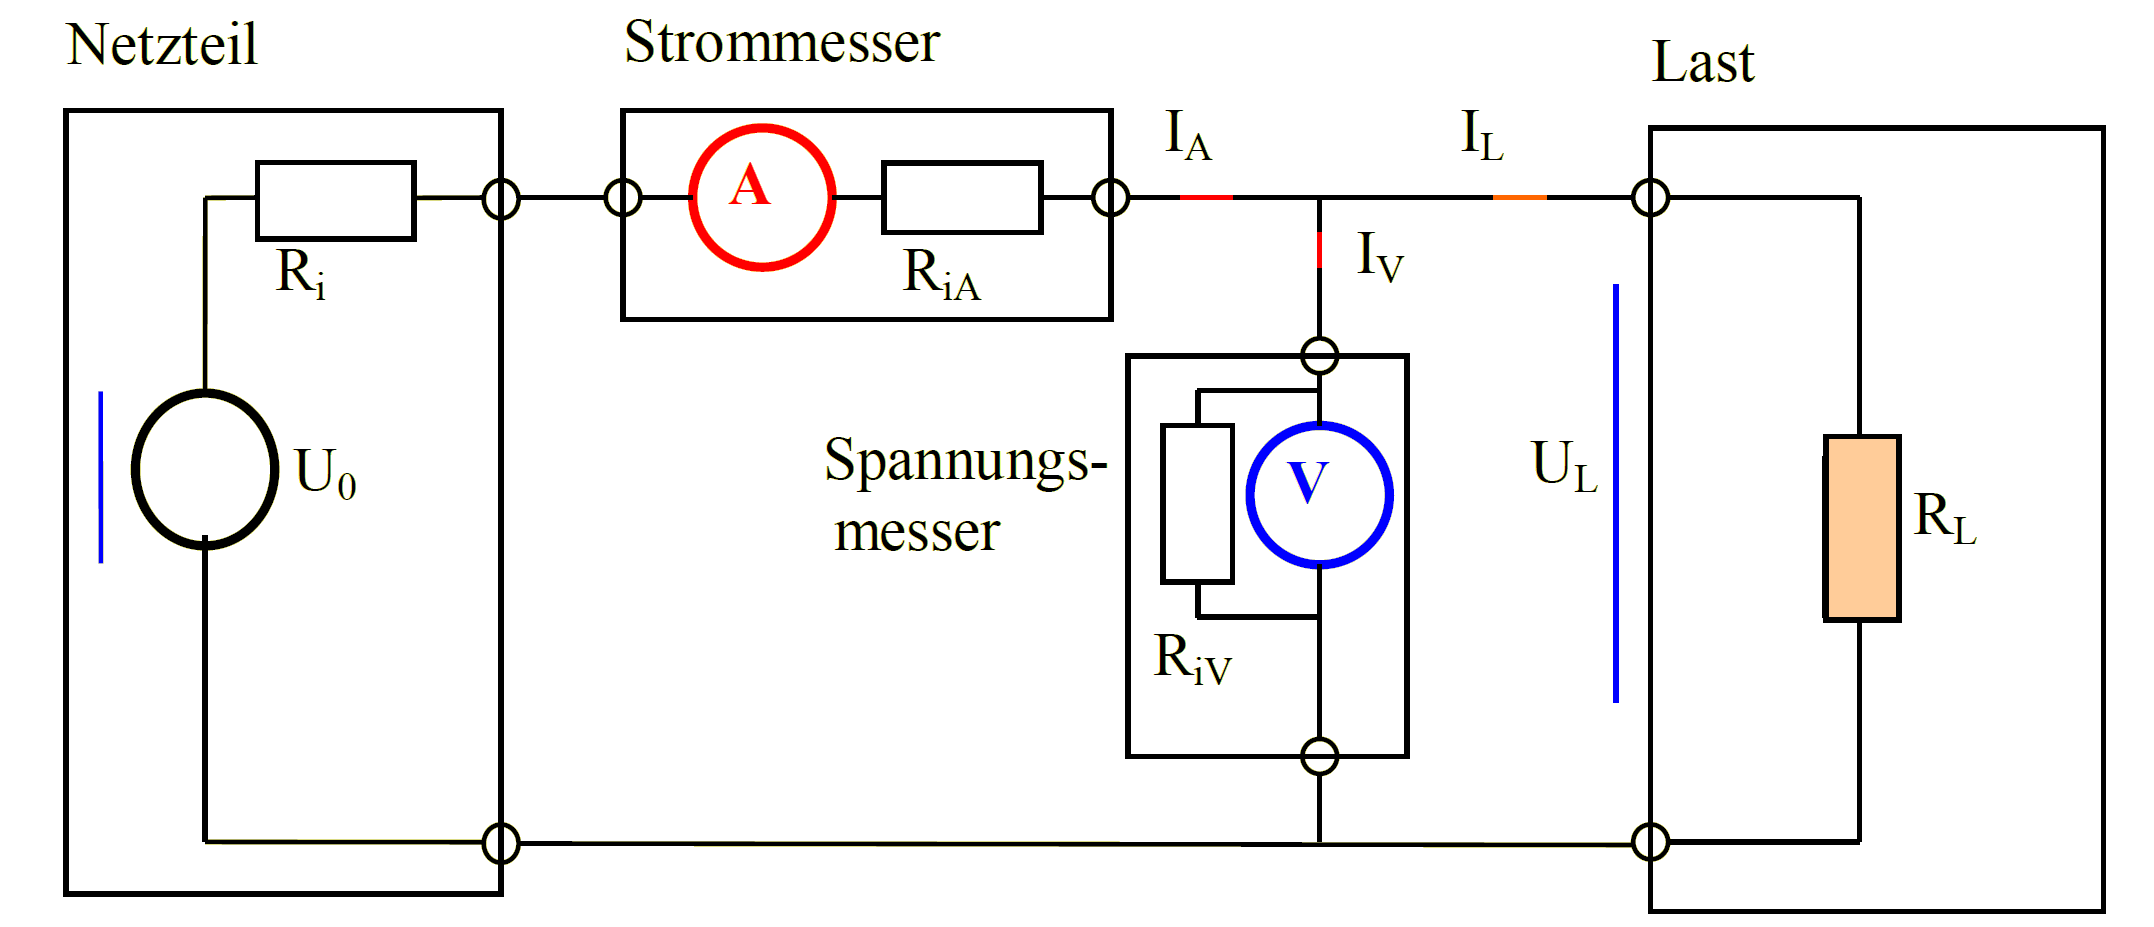
\includegraphics[width=0.8\textwidth]{./Spannung.png}
             \end{center}
         \end{figure}
           
           
           \paragraph{Messfehler} Die Spannung $\spannung{U_L}$ an der Last wird mit dem Spannungsmesser korrekt gemessen und angezeigt. Dagegen zeigt der Strommesser nicht den Strom $\strom{I_L}$ in die Last an, sondern 
           \begin{equation*}
               \strom{I_A} = \strom{I_L} + \strom{I_V}
           \end{equation*}
           
           Der zusätzliche Strom IV kann aus dem angezeigten Wert $\spannung{U_L}$ und aus $\widerstand{R_{iV}}$ bestimmt werden, womit auf den eigentlich interessierenden Strom $\strom{I_L}$ zurückgerechnet werden kann.
            
           
           \subsection{Aufgabe:}  Das Netzteil hat einen Innenwiderstand $\widerstand{R_i} = \SI{1}{\ohm}$. Die Innenwiderstände der Messgeräte sind $\widerstand{R_{iA}} = \SI{100}{\ohm}$ und $\widerstand{R_{iV}} = \SI{1}{\mega\ohm}$ . Die angezeigten Messwerte sind $\spannung{U_L} = \SI{4,95}{\volt}$ und $\strom{I_A} = \SI{500}{\micro\ampere}$.  Berechnen Sie $\strom{I_L}$, $\widerstand{R_L}$ und $\spannung{U_0}$.
           
           
           
         \subsection{Stromrichtige Messung}
         
           \begin{figure}[H]
             \begin{center}
                 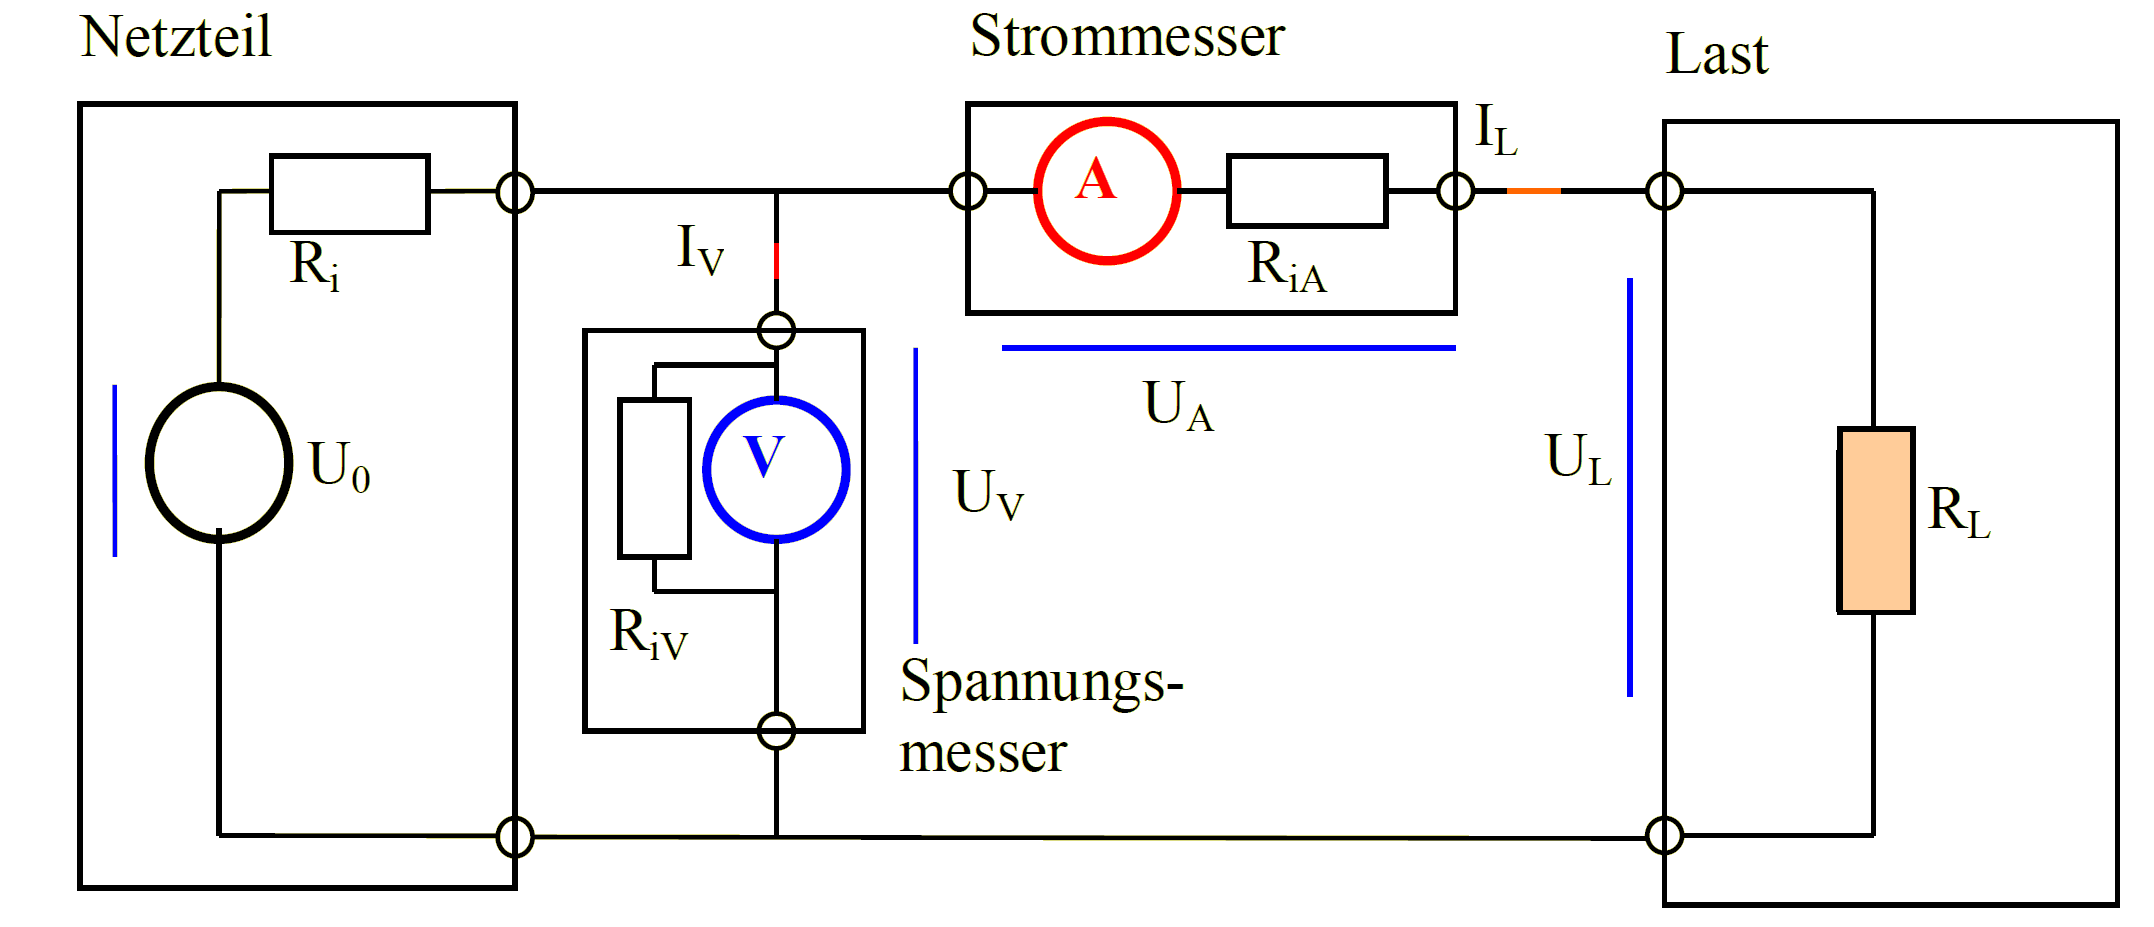
\includegraphics[width=0.8\textwidth]{./Strom.png}
             \end{center}
         \end{figure}
         
         \paragraph{Messfehler}
         Der Strom $\strom{I_L}$ durch die Last wird mit dem Strommesser korrekt gemessen und angezeigt.
         Dagegen zeigt der Spannungsmesser nicht die korrekte Spannung $\spannung{U_L}$ an der Last an, sondern
         \begin{equation*}
             \spannung{U_V} = \spannung{U_L} + \spannung{U_A}
         \end{equation*}
         Die zusätzliche Spannung $\spannung{U_A}$ kann aus dem angezeigten Wert $\strom{I_L}$ und aus $\widerstand{R_{iA}}$ bestimmt
         werden, womit die eigentlich interessierende Spannung $\spannung{U_L}$ berechnet werden kann.
          
          
           \paragraph{Aufgabe:}Das Netzteil hat einen Innenwiderstand $\widerstand{R_i} = \SI{1}{\ohm}$. Die Innenwiderstände der Messgeräte sind $\widerstand{R_{iA}} = \SI{1}{\ohm}$ und $\widerstand{R_{iV}} = \SI{1}{\mega\ohm}$. Die angezeigten Messwerte sind $\spannung{U_L} = \SI{4,8}{\volt}$ und $\strom{I_L} = \SI{100}{\micro\ampere}$. Berechnen Sie  $\strom{U_L}$, $\widerstand{R_L}$ und $\spannung{U_0}$.

		   
       \section{Spannungsrichtiges Messen bei Strom- Spannungs- Messung}
       
         \paragraph{Messaufbau:}
            \begin{itemize*}
                \item 1 Widerstand $\widerstand{R_1}$ = \SI{47}{\ohm}
                \item 1 Widerstand $\widerstand{R_2}$ = \SI{100}{\ohm}
                \item 1 Multimeter Typ M2-H
                \item 1 Multimeter Typ B1020
            \end{itemize*}
            \begin{center}
                \begin{circuitikz}[scale=1]
                    \draw
                    (0,3) to[R, l=$\widerstand{R_1}$, i=$\strom{I_E}$] (2,3)
                          to[short] (3,3)
                    (3,3) to[myammeter, l=M2-H] (5,3)
                    (4,1.5) to[myvoltmeter, l=B1020] (4,0)
                    (3,3) to[open, v_=$\spannung{U_{X1}}$] (3,0)
                    (5,3) to[open, v^=$\spannung{U_{X2}}$] (5,0)
                    
                    (5,3) to[short] (7,3)
                          to[R, l=$\widerstand{R_2}$] (7,0)
                          to[short] (0,0)
                    (0,3) to[open, v=$\spannung{U_V}$] (0,0)
                    
                    (3,3.2) node[] {X1}
                    (5,3.2) node[] {X2}
                    ;
                    \draw [dash pattern=on 4pt off 4pt] (3,3)--(4,1.5);
                    \draw [dash pattern=on 4pt off 4pt] (5,3)--(4,1.5);
                \end{circuitikz}
            \end{center}
            
        \subsection{Messaufgaben}
            \subsubsection{Messaufgabe M1}
            \paragraph{Aufgabe:} Messen und protokollieren Sie die Spannungswerte $\spannung{U_{X1}}$ und $\spannung{U_{X2}}$, sowie die Stromwerte $\strom{I_{X1}}$ und $\strom{I_{X2}}$ bei Spannungsmessung an den Messpunkten $X1$ und $X2$. 
        
            \paragraph{Durchführung:} Messschaltung aufbauen. Betriebsspannung $\spannung{U_V} = \SI{6}{\volt}$ einstellen.
            \paragraph{Ergebnisse:}
                 \begin{center}
                    \begin{table}[H]
                        \caption{Messwertetabelle zur Messaufgabe 2.2.M1}
                        \label{tbl:messergebnisse2.1}
                        \renewcommand{\arraystretch}{1.6}
                        \begin{center}
                            \begin{tabular}{c|c}
                                $\spannung{U_{X1}} [\si{\volt}]$ & \qquad\qquad\qquad\\\hline
                                $\spannung{U_{X2}} [\si{\volt}]$ & \qquad\qquad\qquad\\ \hline
                                $\strom{I_{X1}} [\si{\milli\ampere}]$ & \qquad\qquad\qquad\\\hline
                                $\strom{I_{X2}} [\si{\milli\ampere}]$ & \qquad\qquad\qquad
                            \end{tabular}
                        \end{center}
                    \end{table}
                \end{center}
            
        \subsection{Auswertung}
            \subsubsection{Aufgabe 1:}  An welchem Messpunkt wird bezogen auf den Widerstand $\widerstand{R_2}$ spannungsrichtig gemessen?
            
     
            
            
            \subsubsection{Aufgabe 2:} Berechnen Sie den Innenwiderstand $\widerstand{R_I}$ des Multimeters M2-H im Strommessbereich \SI{60}{\milli\ampere} anhand der Messwerte.
            
            \begin{figure}[H]
                \begin{center}
                    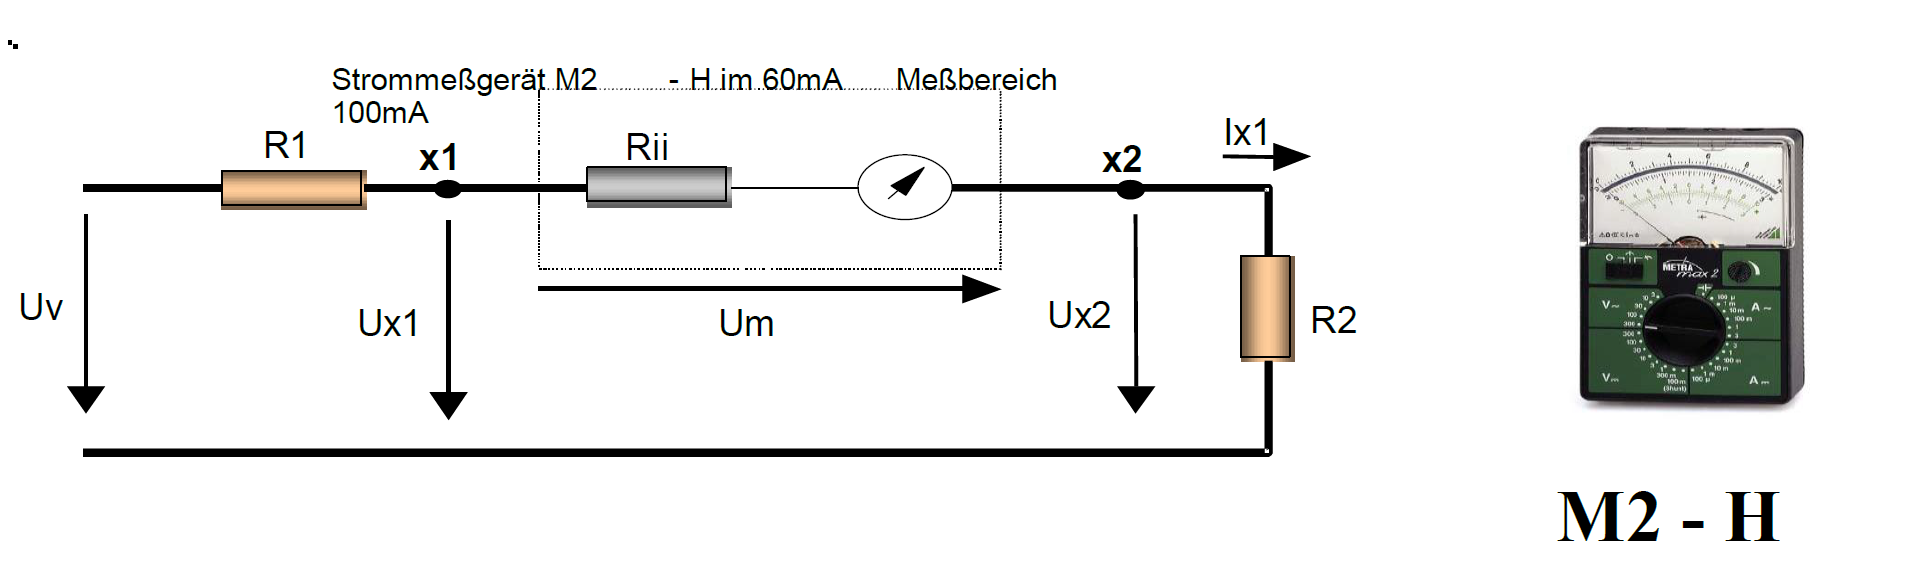
\includegraphics[width=0.8\textwidth]{./M21.png}
                \end{center}
            \end{figure}
        
    
        \section{Stromrichtiges Messen bei gleichzeitiger Strom- Spannungs- Messung}
       
             \paragraph{Messaufbau:}
                \begin{itemize*}
                    \item 1 Widerstand $\widerstand{R_1}$ = \SI{10}{\kilo\ohm}
                    \item 1 Widerstand $\widerstand{R_2}$ = \SI{33}{\kilo\ohm}
                    \item 1 Spannungsmessgerät Typ M2-H
                    \item 1 Strommessgerät Typ B1020
                \end{itemize*}
                \begin{center}
                    \begin{circuitikz}[scale=1]
                        \draw
                        (0,3) to[R, l=$\widerstand{R_1}$, i=$\strom{I_E}$] (2,3)
                        to[short] (3,3)
                        (3,3) to[myammeter, l=B1020] (5,3)
                        (4,1.5) to[myvoltmeter, l=M2-H] (4,0)
                        (3,3) to[open, v_=$\spannung{U_{X1}}$] (3,0)
                        (5,3) to[open, v^=$\spannung{U_{X2}}$] (5,0)
                        
                        (5,3) to[short] (7,3)
                        to[R, l=$\widerstand{R_2}$] (7,0)
                        to[short] (0,0)
                        (0,3) to[open, v=$\spannung{U_V}$] (0,0)
                        
                        (3,3.2) node[] {X1}
                        (5,3.2) node[] {X2}
                        ;
                        \draw [dash pattern=on 4pt off 4pt] (3,3)--(4,1.5);
                        \draw [dash pattern=on 4pt off 4pt] (5,3)--(4,1.5);
                    \end{circuitikz}
                \end{center}
                
            \subsection{Messaufgaben}
                \subsubsection{Messaufgabe M1}
                    \paragraph{Aufgabe:} Messen und protokollieren Sie die Spannungswerte $\spannung{U_{X1}}$ und $\spannung{U_{X2}}$, sowie die Stromwerte $\strom{I_{X1}}$ und $\strom{I_{X2}}$ bei Spannungsmessung an den Messpunkten $X1$ und $X2$. 
                    
                    \paragraph{Durchführung:} Messschaltung aufbauen. Betriebsspannung $\spannung{U_V} = \SI{6}{\volt}$ einstellen
                    \pagebreak
                    \paragraph{Ergebnisse:}
                        \begin{center}
                            \begin{table}[H]
                                \caption{Messwertetabelle zur Messaufgabe 2.3.M1}
                                \label{tbl:messergebnisse2.2}
                                \renewcommand{\arraystretch}{1.6}
                                \begin{center}
                                    \begin{tabular}{c|c}
                                        $\spannung{U_{X1}} [\si{\volt}]$ & \qquad\qquad\qquad\\\hline
                                        $\spannung{U_{X2}} [\si{\volt}]$ & \\ \hline
                                        $\strom{I_{X1}} [\si{\milli\ampere}]$ & \\\hline
                                        $\strom{I_{X2}} [\si{\milli\ampere}]$ & 
                                    \end{tabular}
                                \end{center}
                            \end{table}
                        \end{center}
                  
                
            \subsection{Auswertung}
                \subsubsection{Aufgabe 1:}  An welchem Messpunkt wird bezogen auf den Widerstand $\widerstand{R_2}$ stromrichtig gemessen?
                                
                
                \subsubsection{Aufgabe 2:} Berechnen Sie den Innenwiderstand $\widerstand{R_{UI}}$ des Multimeters M2-H anhand der Messwerte.
                
                $\spannung{U_X}=$ \qquad\qquad\qquad $\strom{I_{X1}}=$ \qquad\qquad\qquad $\strom{I_{X2}}=$
                
                
            \begin{figure}[H]
    \begin{center}
        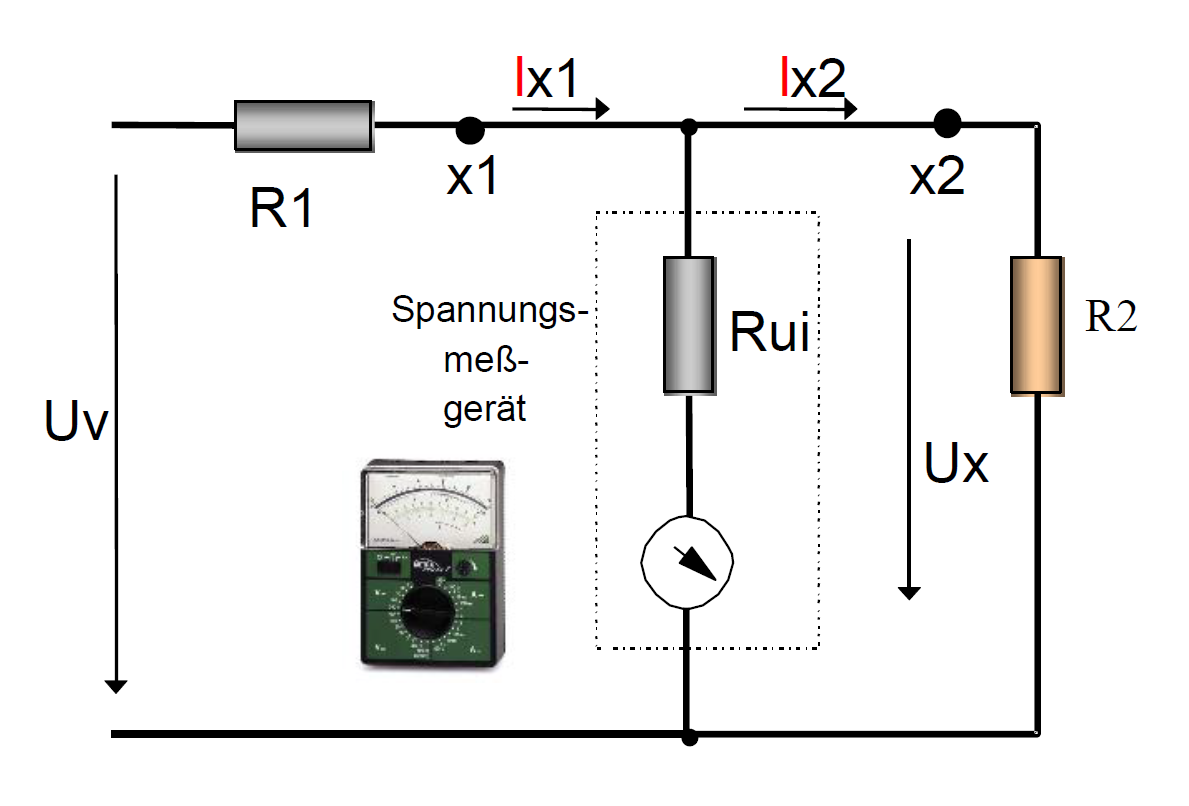
\includegraphics[width=0.6\textwidth]{./M22.png}
    \end{center}
\end{figure}
   
        \section{Einfluss des Messgeräteinnenwiederstandes auf die Messgenauigkeit}
            \paragraph{Messaufbau:}
            \begin{itemize*}
                \item 1 Widerstand $\widerstand{R_1}$ = \SI{100}{\kilo\ohm}
                \item 1 Widerstand $\widerstand{R_2}$ = \SI{100}{\kilo\ohm}
                \item 1 Messgerät Typ M2-H
            \end{itemize*}
            \begin{center}
                \begin{circuitikz}[scale=1]
                    \draw
                    (0,3) to[R, l=$\widerstand{R_1}$, o-] (3,3)
                          to[R, l=$\widerstand{R_2}$, v=$\spannung{U_2}$] (3,0)
                          to[short , -o] (0,0)
    %                (3,3) to[short] (5,3)
   %                       to[R, l=$\widerstand{R_I}$] (5,1.5)
  %                        to[myvoltmeter] (5,0)
                          to[short] (3,0)
%                    (4,3.5) rectangle (6,-0.5)
 %                   (6.7,1.5) node {M2-H}
                    
                    (0,0) to[open, v=$\spannung{U_V}$] (0,3)
                    ;
                \end{circuitikz}
            \end{center}
            
            \subsection{Messaufgaben}
            \subsubsection{Messaufgabe M1}
            \paragraph{Aufgabe:} Zeichnen Sie eine Messschaltung nach obiger Schaltung zur Spannungsmessung an $\widerstand{R_2}$.   Stellen Sie den Spannungsmesser in seinem Ersatzschaltbild dar. Verwenden Sie dazu die Werte aus Übung 2.3 für das Messgerät M2- H. Messen Sie  die Spannung an $\widerstand{R_2}$ 
            \paragraph{Durchführung:} Messschaltung aufbauen. Betriebsspannung $\spannung{U_V} = \SI{6}{\volt}$ einstellen
            \paragraph{Ergebnisse:}
                \begin{align*}
                    \spannung{U_2} = 
                \end{align*}
           
            
            \subsection{Auswertung}
            \subsubsection{Aufgabe 1:}  Erläutern Sie die Ergebnisse aus Messaufgabe 1. Berechnen Sie daraus den Innenwiderstand des Multimeters M2-H im verwendeten Messbereich.
               
            \subsubsection{Aufgabe 2:}  Wie beeinflusst der Innenwiderstand des Spannung- Messgerätes das Messergebnis?
            
               
            \subsubsection{Aufgabe 3:} Zeichnen Sie eine Messschaltung zur Strommessung des Stromes durch $\widerstand{R_2}$ (ohne Spannungsmessung). Stellen Sie den Strommesser in seinem Ersatzschaltbild dar. Verwenden Sie dazu die Werte aus Übung 2.3. für das Messgerät M2-H.
             \
            \subsubsection{Aufgabe 4:} Wie beeinflusst der Innenwiderstand des Strom- Messgerätes die Messung?
            
             
        \section{Kurvenformfehler bei Messgeräten}
        
            \paragraph{Messaufbau:}
            \begin{itemize*}
                \item 1 Widerstand $\widerstand{R}$ = \SI{1}{\kilo\ohm}
                \item 1 Spannungsmessgerät Typ M2-H
                \item 1 Spannungsmessgerät Typ B1020
                \item 1 Oszillograph
                \item 1 Frequenzgenerator
            \end{itemize*}
            \begin{center}
                \begin{circuitikz}[scale=1]
                    \ctikzset{label/align = rotate}
                    \draw
                    (2,3) to[dcvsource, o-o] (2,1)
                    (1,4) to[short] (0,3)
                          to[sV, *-*] (0,1)
                          to[short] (1,0)
                    (1,4) to[short] (4,4)
                          to[R, l=$\widerstand{R}$, v=$\spannung{U}$] (4,0)
                          to[short] (1,0)
                    (6,4) to[myvoltmeter, l=Analog] (6,0)
                    (8,4) to[myammeter, l=Digital] (8,0)
                    (10,4) to[myvoltmeter, l=Oszi] (10,0)
                          
                   ;
                   \draw [dash pattern=on 4pt off 4pt] (1,4)--(2,3);
                   \draw [dash pattern=on 4pt off 4pt] (2,1)--(1,0);
                   \draw [dash pattern=on 6pt off 6pt] (4,4)--(6,4);
                   \draw [dash pattern=on 6pt off 6pt] (4,0)--(6,0);
                   \draw [dash pattern=on 8pt off 8pt] (6,4)--(8,4);
                   \draw [dash pattern=on 8pt off 8pt] (6,0)--(8,0);
                   \draw [dash pattern=on 10pt off 10pt] (8,0)--(10,0);
                   \draw [dash pattern=on 10pt off 10pt] (8,4)--(10,4);
                \end{circuitikz}
            \end{center}
            
            \subsection{Messaufgaben}
            \subsubsection{Messaufgabe M1}
            \paragraph{Aufgabe:} Messen Sie die unten angegebenen Spannungssignale $\spannung{U(t)}$ mit einem analogen und digitalen Messgerät jeweils im Gleich- und Wechselspannungsmessbereich.
            \paragraph{Durchführung:} Messchaltung aufbauen. Versorgungsspannung $\spannung{U(t)}$ mit dem Netzteil (Kurve 1) bzw. dem Frequenzgenerator (Kurve 2 bis 4) einstellen. Messwerte in Tabelle eintragen.\\
            Beachte: Nur immer mit  einem   Messgerät gleichzeitig messen.\\
            			
			Kurvenformen für U(t):            
            \begin{center}
                \begin{table}[H]
                    \caption{Spannungskurven für Messaufgabe 2.5 M1}
                    \label{tbl:kurven2.1}
                    \renewcommand{\arraystretch}{1.3}
                    \begin{center}
                        \begin{tabular}{l|cc}
                            \multicolumn{3}{l}{Kurvenformen für $\spannung{U(t)}$}\\
                            Kurvenform & $U_{SS}$ & $T$\\ \hline
                            \multicolumn{3}{l}{Gleichspannung: (vom Netzteil nehmen)      U =  Umax = 6V}   \\
                            Sinuswechselspannung & 8V & 5ms   \\
                            Dreieckwechselspannung, symm.& 8V & 5ms\\   
                            Rechteckwechselspannung, symm.& 8V &5ms \\
                        \end{tabular}
                    \end{center}
                \end{table}
            \end{center}            
             

            
            ($U_{ss}$, $U_{pp}$ = U Spitze/Spitze oder 2 * Û) 
            \paragraph{Ergebnisse:}
            \begin{center}
                \begin{table}[H]
                    \caption{Messwertetabelle zur Messaufgabe 2.3.M1}
                    \label{tbl:messergebnisse2.2}
                    \renewcommand{\arraystretch}{1.6}
                    \begin{center}
                        \begin{tabular}{c|cc|c|c|c|c}
                            Messgerät & Messprinzip & Messbereich & Gleichspannung & Sinuskurve & Dreieck & Rechteck\\ \hline
                            M2-H & Drehspul & 6\,V\textdirectcurrent &  &  &  & \\\hline
                            M2-H & Drehspul & 6\,V$\sim$ &  &  &  & \\\hline
                            B1020 & Digital & 6\,V\textdirectcurrent & &  &  & \\\hline
                            B1020 & Digital & 6\,V$\sim$ &  &  &  & \\
                            
                        \end{tabular}
                    \end{center}
                \end{table}
            \end{center}
            
            \subsection{Auswertung}
            \subsubsection{Aufgabe 1:} Wie kommt der Formfaktor F für Sinusgrößen zustande (math. Herleitung) 
    
            
            \subsubsection{Aufgabe 2:} Was messen Sie mit den Multimetern im Gleichspannungsbereich, was im   Wechselspannungsbereich? Warum? 

		
            \subsubsection{Aufgabe 3:} Wie kommen die Anzeigewerte für Dreieck- und Rechteckspannung zustande ?   (Rechnung)\\
            
            \subsubsection{Aufgabe 4:} Berechnen Sie aus den Anzeigewerten die tatsächlichen Effektivwerte für die   obige Dreieck- und Rechteckspannung. Geben Sie die Umrechnungsfaktoren an.
            
    \chapter{Kennwerte harmonischer Wechselgrößen}
     
        \section{Rechenaufgaben}
            \subsection{Aufgabe 1:}
                 Eine sinusförmige Spannung $\spannung{U(t)}$ mit $f_1 = \SI{50}{\hertz}$ hat den Scheitelwert $\hat{U} = \SI{10}{\volt}$
                 
                 a) Beschreiben Sie die Funktion $\spannung{U(t)}$
                 
                 b) Wie groß ist  $\spannung{U(t)}$ bei $t_1 = \SI{2}{\milli\second}$ nach dem Nulldurchgang?
                 
                 c) Skizzieren Sie das einseitige Spektrum $\spannung{U(f)}$
                 
                 d)Wie groß wäre die Phase $\varphi$, wenn der Nulldurchgang bei $t_2 = \SI{5}{\milli\second}$ ist, wie lautet dann $\spannung{U(t)}$? 
               
                
        \section{Speisung eines ohmschen Verbrauchers mit einer Sinusspannung}
            \paragraph{Messaufbau:}
                \begin{itemize*}
                    \item 1 Widerstand $\widerstand{R_1}$ = \SI{1}{\kilo\ohm}
                    \item 1 Widerstand $\widerstand{R_m}$ = \SI{100}{\ohm}
                \end{itemize*}
                \begin{center}
                    \begin{circuitikz}[scale=1.2]
                        \draw
                       (0,4) to[myammeter, i=$\strom{I}$] (2,4)
                             to[short] (4,4)
                             to[R, l=$\widerstand{R_1}$, v=$\spannung{U_1}$] (4,2)
                             to[R, l=$\widerstand{R_m}$, v=$\spannung{U_m}$] (4,0)
                             to[short] (0,0)
                        (2,4) to[myvoltmeter, v=$\spannung{U}$] (2,0)
                        (4,4) to[short] (6,4) to[short] (6,3.4)
                        (4,2) to[short] (6,2) to[short] (6,2.6)
                        (4,0) to[short] (7,0) to[short] (7,3) to[short] (6.5,3) 
                        (5.5,2) to[myvoltmeter] (5.5,0)
                        (0,4) to[sV, v_=$\spannung{U(t)}$] (0,0)
                        (6.5,3) node[oscillator]{}
                        (5,4.25) node{Kanal1}
                        (5,2.25) node{Kanal2}
                        (7,3.25) node{Oszi}
                        (6,-0.25) node{Gnd}
                        ;
                    \end{circuitikz}
                \end{center}
            
            \subsection{Messaufgaben}
                \subsubsection{Messaufgabe M1}
                    \paragraph{Aufgabe:} Messen Sie mit dem Multimeter:\\
                     $\spannung{U}=$\\
                      $\strom{I}=$\\
                      $\spannung{U_m}=$\\
                     Messen Sie mit dem Oszillograph den Phasenwinkel $\varphi(\spannung{u},\strom{I})$ für 10 Augenblickwerte für $\spannung{U(t)}$ und $\strom{I(t)}$ = $\frac{\spannung{U_m(t)}}{\widerstand{R}}$
                    \paragraph{Durchführung:} Schaltung aufbauen. Die Speisespannung $\spannung{U(t)}$ am Frequenzgenerator einstellen: Spannung $U_{SS} = \SI{8}{\volt}$, Periodendauer  $T = \SI{10}{\milli\second}$ 
                    \paragraph{Ergebnisse:}
                        \begin{center}
                            \begin{table}[H]
                                \caption{Messwertetabelle zur Messaufgabe 3.2.M1}
                                \label{tbl:messergebnisse3.1}
                                \renewcommand{\arraystretch}{1.6}
                                \begin{center}
                                    \begin{tabular}{c|c|c|c|c}
  										 $t \quad [\si{\milli\second}]$ & $\spannung{U(t)}\quad  [\si{\volt}]$ & $\spannung{U_m} \quad [\si{\milli\volt}]$ & $\strom{I(t)} = \frac{\spannung{U_m}}{\widerstand{R_m}}  \quad[\si{\milli\ampere}]$ & $P(t) \quad [\si{\milli\watt}]$\\ \hline
   										 \qquad\qquad\qquad& \qquad\qquad\qquad & \qquad\qquad\qquad & \qquad\qquad\qquad  & \qquad\qquad\qquad\\\hline
   										 &  &  &  & \\\hline
   										 &  &  &  & \\\hline
   										 &  &  &  & \\\hline
  										 &  &  &  & \\\hline
   										 &  &  &  & \\\hline
   										 &  &  &  & \\\hline
   										 &  &  &  & \\\hline
   										 &  &  &  & \\\hline
   										 &  &  &  & \\
									\end{tabular}
                                \end{center}
                            \end{table}
                        \end{center}
                    
            
            \subsection{Auswertung}
                \subsubsection{Aufgabe 1:}  Berechnen Sie zu den einzelnen Punkten die momentane Leistung $P(t) = \spannung{U(t)} \cdot \strom{I(t)}$ 

                \subsubsection{Aufgabe 2:}   Stellen Sie $\spannung{U(t)}$, $\strom{I(t)}$ und $P(t)$ graphisch dar.(In einer Zeichnung, verschieden farbig)
                
                \subsubsection{Aufgabe 3:}  Was messen Sie mit den Strom- und Spannungsmessern im Wechselstrombereich ? Welche Leistung können Sie daraus berechnen. (Multimeter benutzen)
               
                \subsubsection{Aufgabe 4:}   Erläutern Sie die Begriffe Schein-, Blind- und Wirkleistung.   P=?; Q=?; S=?
      
                         
                         
                
                 
        \section{Speisung eines kapazitiven Verbrauchers mit einer Sinusspannung}
            \paragraph{Messaufbau:}
                \begin{itemize*}
                    \item 1 Kondensator $\capacity{C} = \SI{0,1}{\micro\farad}, \SI{40}{\volt}$
                    \item 1 Widerstand $\widerstand{R_M} = \SI{100}{\ohm}$
                \end{itemize*}
                \begin{center}
                    \begin{circuitikz}[scale=1]
                        \draw
                        (0,0) to[sV, v=$\spannung{U(t)}$] (0,4)
                              to[short, i=$\strom{I}$] (4,4)
                              to[C, l=$\capacity{C}$, v=$\spannung{U_C}$] (4,2)
                              to[R, l=$\widerstand{R_M}$, v=$\spannung{U_M}$] (4,0)
                              to[short, l=Gnd] (0,0)
                        (4,4) to[short, l=Kanal 1] (6,4)
                        (4,2) to[short, l=Kanal 2] (6,2)
                                                     
                        ;
                    \end{circuitikz}
                \end{center}
            
            \subsection{Messaufgaben}
                \subsubsection{Messaufgabe M1}
                   \paragraph{Aufgabe:} Messen Sie mit dem Multimeter:
                   
                   $\spannung{U}=$
                   
                   $\strom{I}=$
                   
                   $\spannung{U_m}=$
                   
                   Messen Sie mit dem Oszillograph den Phasenwinkel $\varphi(\spannung{u},\strom{I})$ für 10 Augenblickwerte für $\spannung{U(t)}$ und $\strom{I(t)}$ = $\frac{\spannung{U_m(t)}}{\widerstand{R}}$
                   \paragraph{Durchführung:} Schaltung aufbauen. Die Speisespannung $\spannung{U(t)}$ am Frequenzgenerator einstellen: Spannung $U_{SS} = \SI{8}{\volt}$, Periodendauer  $T = \SI{10}{\milli\second}$ 
                   \paragraph{Ergebnisse:}
                   \begin{center}
                       \begin{table}[!hbtp]
                           \caption{Messwertetabelle zur Messaufgabe 3.3.M1}
                           \label{tbl:messergebnisse3.1}
                           \renewcommand{\arraystretch}{1.6}
                           \begin{center}
                               \begin{tabular}{c|c|c|c|c|c}
									$t [\si{\milli\second}]$ & $\spannung{U(t)} [\si{\volt}]$ & $\spannung{U_m} [\si{\milli\volt}]$ & $\strom{I(t)} = \frac{\spannung{U_m}}{\widerstand{R_m}} [\si{\milli\ampere}]$ & $\phi [°]$ & $P(t) [\si{\milli\watt}]$\\ \hline
									\qquad\qquad\qquad & \qquad\qquad\qquad & \qquad\qquad\qquad & \qquad\qquad\qquad & \qquad\qquad\qquad & \qquad\qquad\qquad\\\hline
									 &  &  &  &  & \\\hline
									 &  &  &  &  & \\\hline
									 &  &  &  &  & \\\hline
									 &  &  &  &  & \\\hline
									 &  &  &  &  & \\\hline
									 &  &  &  &  & \\\hline
									 &  &  &  &  & \\\hline
									 &  &  &  &  & \\\hline
									 &  &  &  &  & \\
							   \end{tabular}
                           \end{center}
                       \end{table}
                   \end{center}
                   
                   
                   \subsection{Auswertung}
                   \subsubsection{Aufgabe 1:}  Berechnen Sie zu den einzelnen Punkten die momentane Leistung $P(t) = \spannung{U(t)} \cdot \strom{I(t)}$ 

                   \subsubsection{Aufgabe 2:}   Stellen Sie $\spannung{U(t)}$, $\strom{I(t)}$ und $P(t)$ graphisch dar.(In einer Zeichnung, verschieden farbig)
                   
                              
        \section{Bestimmen der Größe eines Kondensators anhand der Auf- bzw. Entladekurve}
        
            \paragraph{Messaufbau:}
               \begin{itemize*}
                   \item 1 Kondensator $\capacity{C} = ?$
                   \item 1 Widerstand $\widerstand{R} = \SI{10}{\kilo\ohm}$
               \end{itemize*}
               \begin{center}
                   \begin{circuitikz}[scale=1]
                       \draw
                       (0,0) to[sV, v=$\spannung{U(t)}$] (0,4)
                       to[short, i=$\strom{I}$] (4,4)
                       to[C, l=$\capacity{C}$, v=$\spannung{U_C}$] (4,2)
                       to[R, l=$\widerstand{R}$, v=$\spannung{U_R}$] (4,0)
                       to[short, l=Gnd] (0,0)
                       (4,4) to[short, l=Kanal 1] (6,4)
                       (4,2) to[short, l=Kanal 2] (6,2)
                       
                       ;
                   \end{circuitikz}
               \end{center}
            
            \subsection{Messaufgaben}
                \subsubsection{Messaufgabe M1}
                    \paragraph{Durchführung:}Schaltung aufbauen. Die Speisespannung u(t) am Frequenzgenerator einstellen:\\
					$\spannung{U_{ss}}$ (Spitze/Spitze) = $\SI{4}{\volt}$\\
					Periodendauer T = ?
                    \paragraph{Aufgabe:}Bestimmen Sie die Ihrer Meinung nach beste Art (Sinus, Dreieck, Rechteck) und Größe der Frequenz (Hz, kHz, MHz), um eine gut sichtbare Auf- bzw. Entladekurve
darzustellen und somit die Größe des Kondensators berechnen zu können. Geben Sie
die gewählte Art an.

            		\paragraph{Ergebnisse:}
            		\begin{center}
                       \begin{table}[H]
                           \caption{Messwertetabelle zur Messaufgabe 3.4.M1}
                           \label{tbl:messergebnisse3.4}
                           \renewcommand{\arraystretch}{1.6}
                           \begin{center}
                               \begin{tabular}{c|c|c|c}
									Art & $f$ & t Aufladung & t Entladung\\ \hline
									\qquad\qquad\qquad & \qquad\qquad\qquad & \qquad\qquad\qquad & \qquad\qquad\qquad
							   \end{tabular}
                           \end{center}
                       \end{table}
                   \end{center}
            \subsection{Auswertung}
                \paragraph{Aufgabe 1:}Auf- und Entladekurve graphisch darstellen. Berechnen Sie aus den Messwerten die Größe des Kondensators. Mathematische Darstellung der Berechnung.
                	  
\end{document}
